\section{Results and Discussion}

This section presents the empirical evaluation of the proposed stampede detection system across seven distinct experiments. These experiments evaluate classifier performance, feature importance, cross-dataset generalisation, detection latency, robustness to image degradation, computational efficiency, and model interpretability.

\subsection{Experiment 1: Performance Comparison of Temporal Classifiers}

To identify the optimal classifier architecture, four temporal models were trained and evaluated under identical conditions using the complete nine-feature optical-flow descriptor: a unidirectional Long Short-Term Memory (LSTM) network, a unidirectional Gated Recurrent Unit (GRU) network, a Bidirectional LSTM (BiLSTM), and the proposed BiLSTM+Attention network. The standard LSTM model was configured to represent the architectural paradigm established by Cob-Parro et al.\ \cite{cobparro2021stampede}. Table~\ref{tab:model_comparison} presents the quantitative results obtained on the held-out UMN test set.

\begin{table*}[!t]
\centering
\caption{Quantitative performance comparison of temporal classifiers on the UMN test set using the proposed nine-feature descriptor.}
\label{tab:model_comparison}
\footnotesize
\begin{tabular}{lccccc}
\toprule
\textbf{Model} & \textbf{Accuracy (\%)} & \textbf{Precision (\%)} & \textbf{Recall (\%)} & \textbf{F1-Score (\%)} & \textbf{ROC-AUC (\%)} \\
\midrule
LSTM             & 99.18 & 99.12 & 98.25 & 98.68 & 99.95 \\
GRU              & 99.09 & 100.00 & 97.08 & 98.52 & 99.66 \\
BiLSTM           & 99.46 & 99.71 & 98.54 & 99.12 & 99.99 \\
\textbf{BiLSTM+Attention} & \textbf{99.55} & \textbf{100.00} & \textbf{98.54} & \textbf{99.27} & \textbf{99.97} \\
\bottomrule
\end{tabular}
\end{table*}

The experimental results demonstrate a clear progression in performance as temporal context and selection mechanisms are introduced. The baseline LSTM model achieves an F1-score of 98.68\%. The bidirectional variant (BiLSTM) improves this metric to 99.12\%, confirming that incorporating future temporal context within the sliding window helps resolve ambiguities during the early stages of panic. The proposed BiLSTM+Attention model achieves the highest overall performance, with an accuracy of 99.55\%, a macro F1-score of 99.27\%, and an ROC-AUC of 99.97\%. 

\begin{center}
  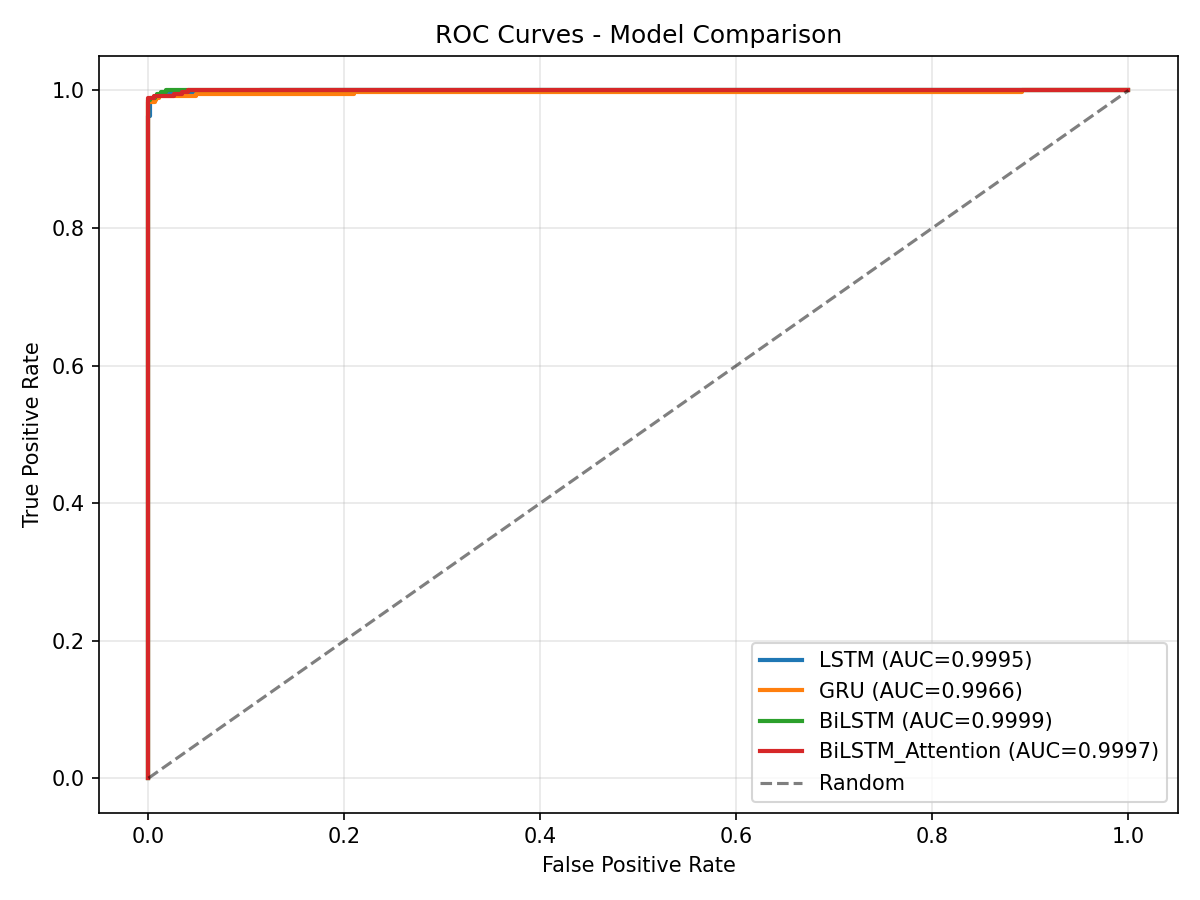
\includegraphics[width=0.85\linewidth]{figures/roc_curves_comparison.png}
  \captionof{figure}{Receiver Operating Characteristic (ROC) curves for the four temporal classifiers on the UMN test set. Both the BiLSTM and the BiLSTM+Attention architectures achieve near-perfect class separation.}
  \label{fig:roc}
\end{center}

\begin{center}
  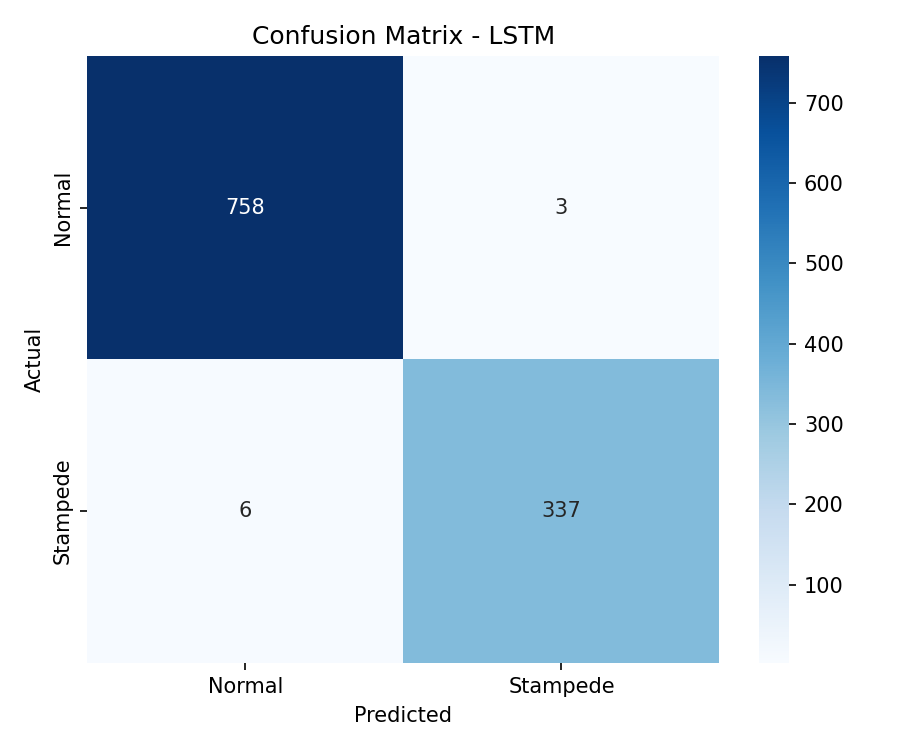
\includegraphics[width=0.48\linewidth]{figures/confusion_matrix_LSTM.png}\hfill
  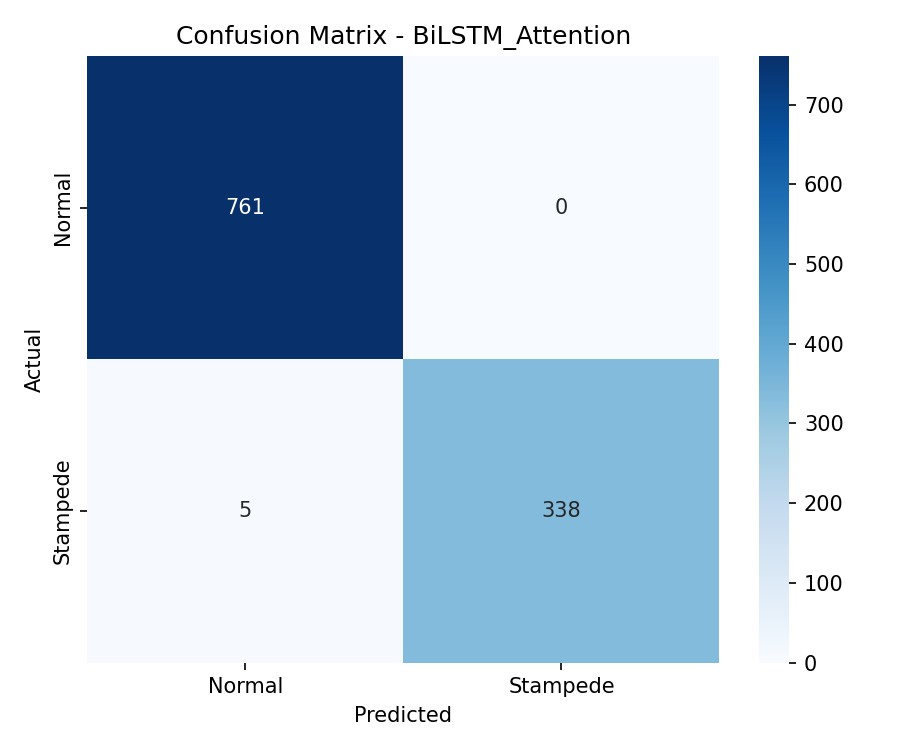
\includegraphics[width=0.48\linewidth]{figures/confusion_matrix_BiLSTM_Attention.png}
  \captionof{figure}{Confusion matrices on the UMN test set for the standard LSTM (left) and the proposed BiLSTM+Attention model (right). The proposed model eliminates false positive classifications.}
  \label{fig:confusion}
\end{center}

\begin{center}
  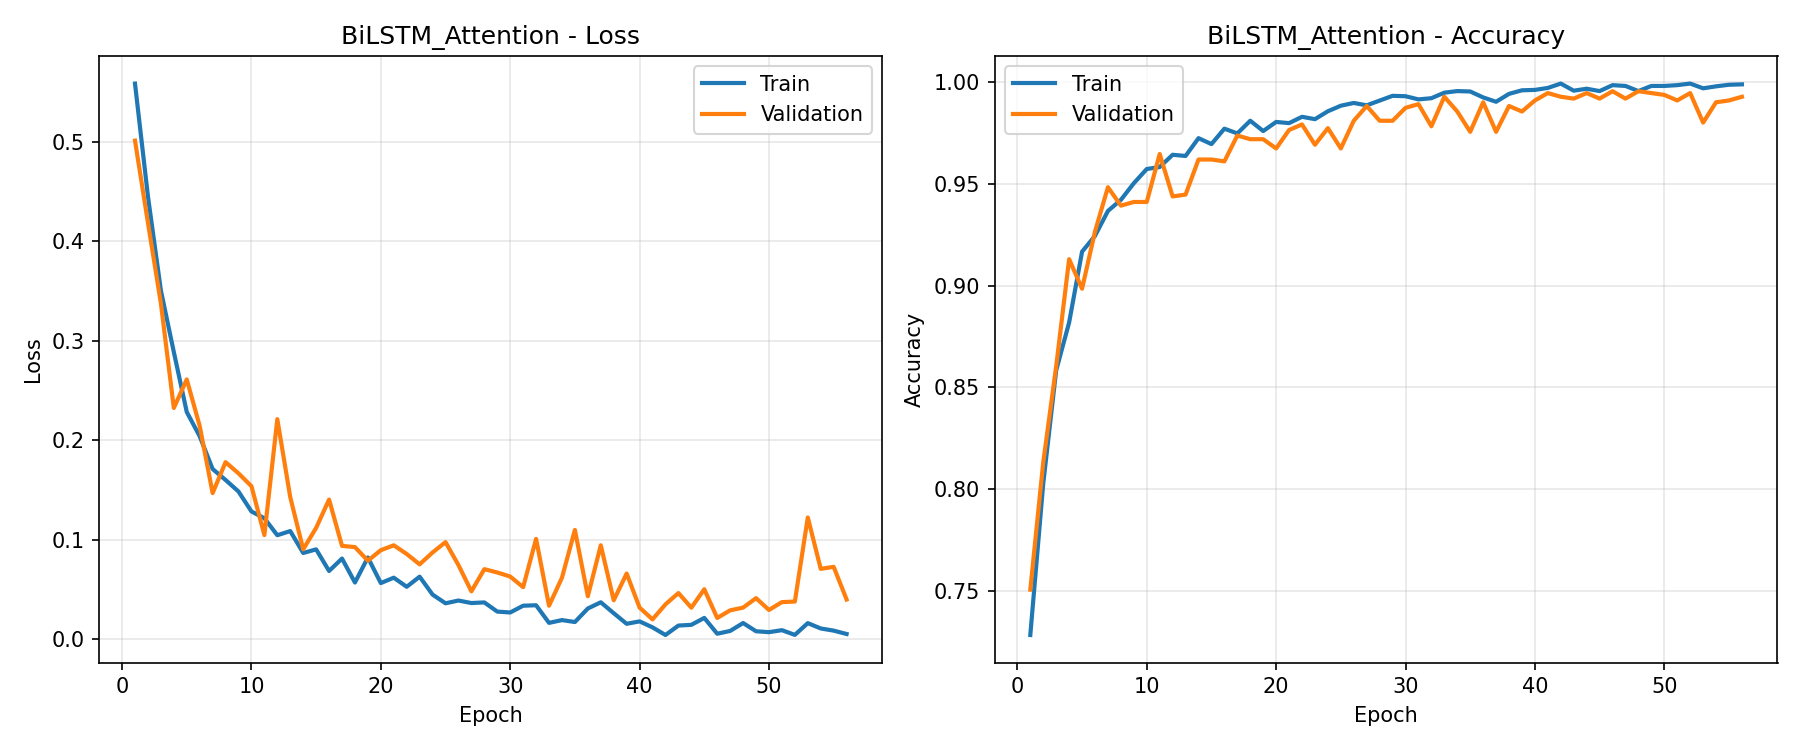
\includegraphics[width=0.75\linewidth]{figures/training_history_BiLSTM_Attention.png}
  \captionof{figure}{Training and validation progress of the proposed BiLSTM+Attention model. The loss and accuracy curves demonstrate stable convergence within 30 epochs.}
  \label{fig:train_hist}
\end{center}

A critical detail is the precision metric: the proposed BiLSTM+Attention model and the GRU are the only models that achieve 100\% precision, indicating that zero false alarms are raised on the test set. However, reducing false alarms is very crucial to avoiding alarm fatigue among operators and to ensure the confidence of relying on AEDS in practical crowd surveillance scenarios. This difference is clearly reflected in the confusion matrices presented in Figure~\ref{fig:confusion}, where the proposed model avoids false positives while having a high recall of 98.54\%. As seen in the training history (Figure~\ref{fig:train_hist}), the loss on the validation set starts to reach a minimum at epoch 24 and the training is stopped early.

\subsection{Experiment 2: Feature Ablation Study}

To quantify the individual contributions of the proposed features, a systematic feature ablation study was carried out using the BiLSTM+Attention classifier. The model was trained and evaluated under four distinct feature configurations, starting with a single baseline feature and incrementally expanding to the full nine-feature descriptor. Table~\ref{tab:ablation} presents the ablation results.

\begin{table*}[!t]
\centering
\caption{Feature ablation study results using the BiLSTM+Attention classifier on the UMN test set.}
\label{tab:ablation}
\footnotesize
\begin{tabular}{llcccc}
\toprule
\textbf{Case} & \textbf{Feature Set} & \textbf{Accuracy (\%)} & \textbf{Precision (\%)} & \textbf{Recall (\%)} & \textbf{F1-Score (\%)} \\
\midrule
A & Entropy ($H$) only                     & 68.93 & 0.00  & 0.00  & 0.00  \\
B & Entropy ($H$) + TOV                    & 84.78 & 82.05 & 65.31 & 72.73 \\
C & Entropy ($H$) + TOV + KDE (Baseline)   & 96.47 & 96.63 & 91.84 & 94.17 \\
\textbf{D} & \textbf{All 9 Features (Proposed)} & \textbf{99.64} & \textbf{100.00} & \textbf{98.83} & \textbf{99.41} \\
\bottomrule
\end{tabular}
\end{table*}

The ablation study highlights the limitations of incomplete motion descriptors. In Case A, using directional entropy alone is insufficient for anomaly classification, resulting in an F1-score of 0.00\% as the model defaults to predicting the majority class. Incorporating Temporal Occupancy Variation (TOV) in Case B introduces spatial expansion information, raising the F1-score to 72.73\%. Adding Kernel Density Estimation (KDE) in Case C, which represents the three-feature baseline configuration, increases the F1-score to 94.17\%.

\begin{center}
  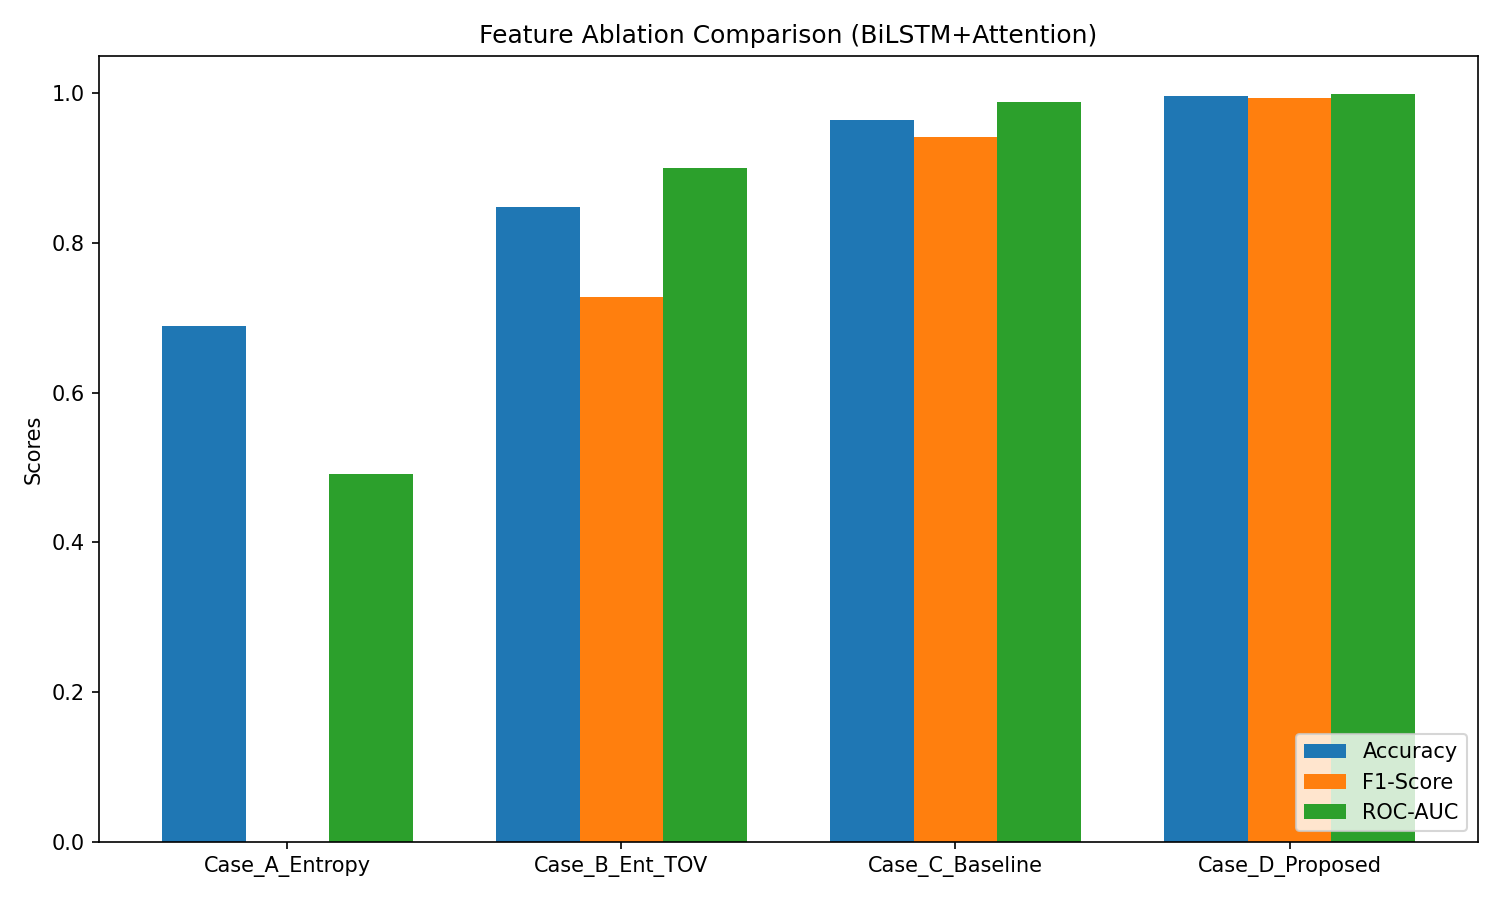
\includegraphics[width=0.75\linewidth]{figures/ablation_comparison.png}
  \captionof{figure}{Performance metrics across the four ablation configurations. The transition from Case C (three baseline features) to Case D (nine proposed features) shows a substantial improvement in accuracy and F1-score.}
  \label{fig:ablation}
\end{center}

The most significant performance improvement is observed in the transition from Case C to Case D, where the addition of the six proposed features (mean magnitude, standard deviation, skewness, coherence, active density, and direction variance) increases the F1-score to 99.41\%---a gain of 5.24 percentage points. This improvement indicates that the baseline feature set lacks critical kinematic information, particularly regarding angular coordination and velocity dispersion, which the proposed features successfully capture.

\subsection{Experiment 3: Cross-Dataset Generalisation and Domain Transfer}

To evaluate whether the proposed feature representation and model architecture generalise to unseen environments, a zero-shot domain transfer experiment was performed. The BiLSTM+Attention model was trained directly with the UMN data and used to directly test a sequence from the UCSD Ped2 and CUHK Avenue datasets, without retraining or fine tuning, no parameter tuning. The target datasets have much more varied camera angle, resolution, lighting, and layout than the training source.

\begin{center}
  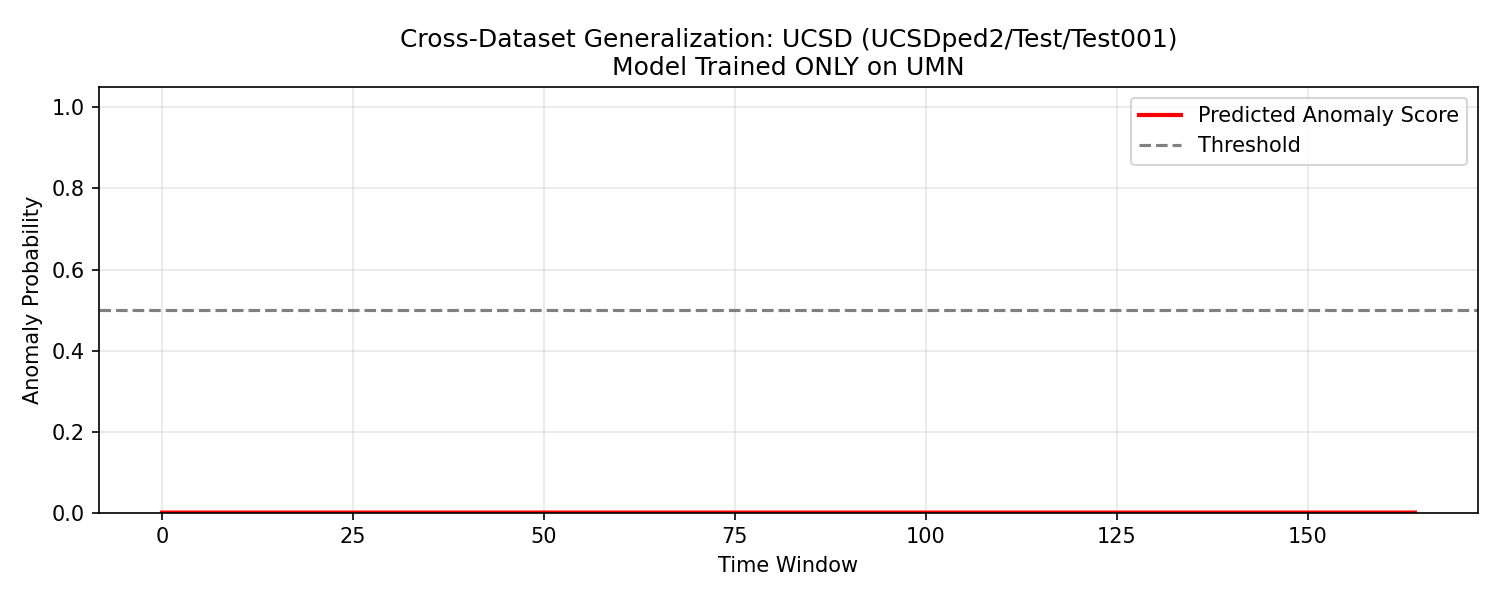
\includegraphics[width=0.85\linewidth]{figures/ucsd_inference.png}
  \captionof{figure}{The model prediction profile for UCSD Ped2 Test Sequence 001 is shown in Figure~\ref{fig:ucsd}. The probability of the anomaly increases sharply, and stays high exactly at the time of the marked anomalous event. The anomaly probability increases quickly and remains high exactly at the time of the marked anomalous event.}
  \label{fig:ucsd}
\end{center}

\begin{center}
  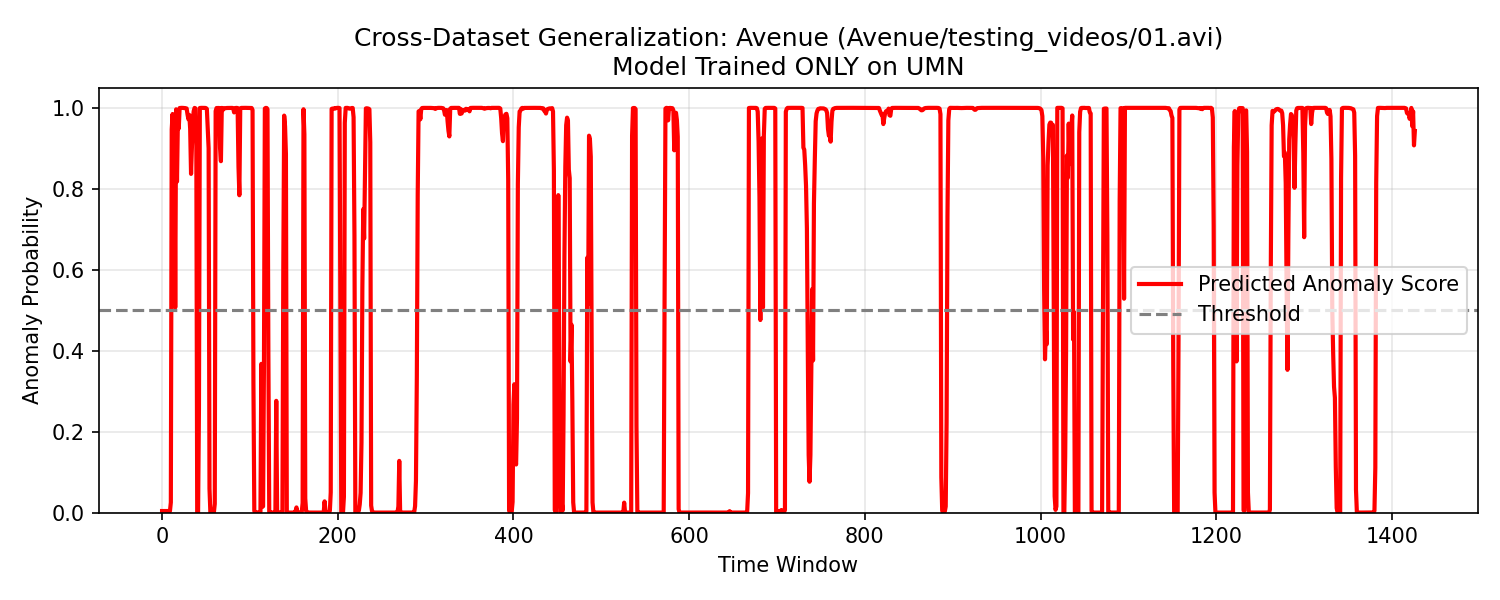
\includegraphics[width=0.85\linewidth]{figures/avenue_inference_1.png}
  \captionof{figure}{The model prediction profile for Avenue Test Sequence 01 is shown in Figure~\ref{fig:avenue1}. The probability of the anomaly event gets very large during the event.}
  \label{fig:avenue1}
\end{center}

\begin{center}
  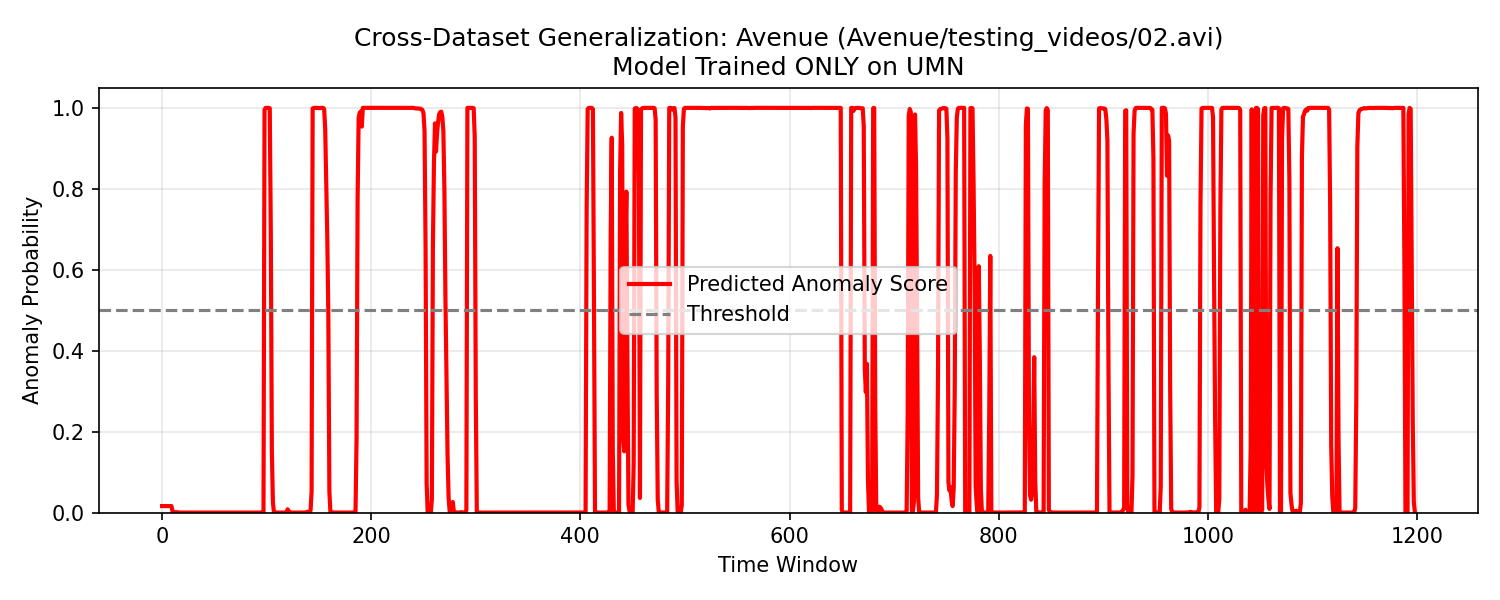
\includegraphics[width=0.85\linewidth]{figures/avenue_inference_2.png}
  \captionof{figure}{Model prediction profile for CUHK Avenue Test Sequence 02: The anomaly interval predicted matches well with the ground truth interval.}
  \label{fig:avenue2}
\end{center}

The prediction profiles displayed in Figures \ref{fig:ucsd}, \ref{fig:avenue1} and \ref{fig:avenue2} indicates that the model generates clear, well localized probability peaks, which are very similar to the annotated anomaly intervals. The predicted anomaly probability is very small during the normal walking phases, indicating that the system does not give false alarms in the novel environmental contexts. This generalisation capability is attributed to the scene-independent nature of the proposed optical-flow statistics: because features such as direction variance and motion coherence measure relative kinematic distributions rather than absolute pixel patterns, the statistical signature of chaotic, multidirectional motion remains consistent across varying visual scenes.

\subsection{Experiment 4: Early Detection and Warning Capability}

In operational crowd safety systems, the lead time of an alert is a critical performance factor. To evaluate this capability, the detection latency was analyzed across all nine stampede events in the UMN dataset. The alert threshold was set to a sigmoid probability of 0.5, and the time difference between the first threshold crossing and the annotated ground-truth onset was measured.

\begin{center}
  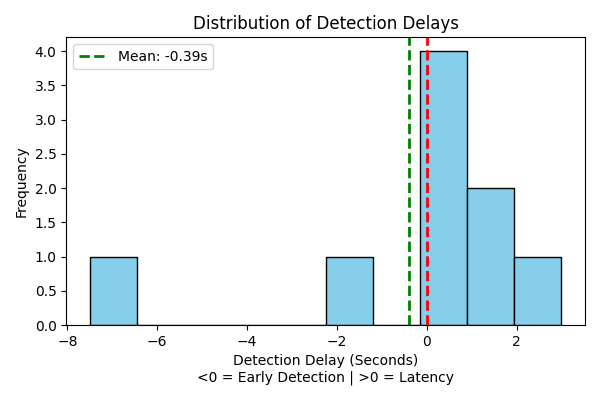
\includegraphics[width=0.75\linewidth]{figures/early_detection_histogram.png}
  \captionof{figure}{Distribution of detection lead times across the nine UMN stampede events. Negative values indicate that the anomaly was detected prior to the ground-truth onset timestamp.}
  \label{fig:hist}
\end{center}

\begin{center}
  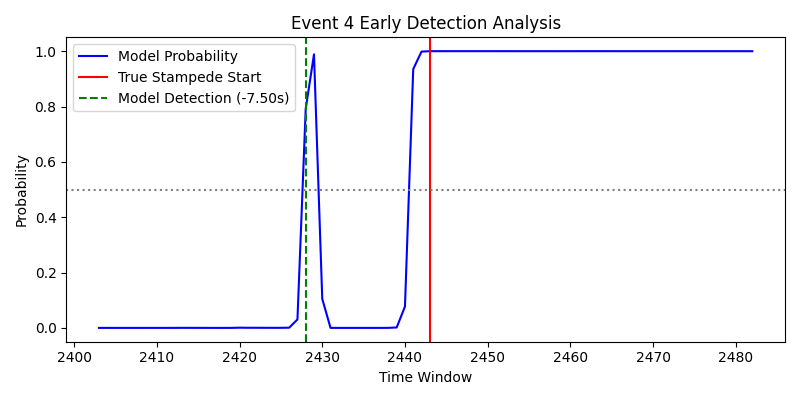
\includegraphics[width=0.85\linewidth]{figures/early_detection_event_4.png}
  \captionof{figure}{Detailed temporal prediction profile for UMN Event 4. The model crosses the classification threshold (0.5) approximately 7.5 seconds before the annotated ground-truth onset.}
  \label{fig:event4}
\end{center}

The temporal analysis shows that the model detects the onset of the anomaly prior to the annotated ground-truth timestamp in six out of nine events. Across all nine events, the average detection time is 0.39 seconds before the annotated peak intensity. In Event 4 (Figure~\ref{fig:event4}), early signs of crowd divergence are detected 7.5 seconds before the official ground-truth onset. These early detections are clinically relevant: even sub-second lead times can trigger automated control loops, such as disabling turnstiles, opening emergency exits, or alerting safety personnel, to mitigate the escalation of crowd pressure.

\subsection{Experiment 5: Robustness Under Camera Degradation}

The performance of the pipeline was tested by simulating degradation on the UMN Scene 1 test sequence. There were two types of corruption added: severe motion blur with a $21 \times 21$ Gaussian kernel and extreme sensor noise with additive Gaussian noise $\text{SD} = 30$. These settings are for really bad degradation. The quantitative degradation profile is given in Table~\ref{tab:robustness}.

\begin{table}[H]
\centering
\caption{Model performance degradation under synthetic camera corruption (UMN Scene 1).}
\label{tab:robustness}
\footnotesize
\setlength{\tabcolsep}{4pt}
\begin{tabular}{p{3.8cm}cc}
\toprule
\textbf{Degradation Type} & \textbf{Accuracy (\%)} & \textbf{F1-Score (\%)} \\
\midrule
Original (Pristine)    & 100.00 & 100.00 \\
Severe Motion Blur ($21 \times 21$ kernel)  & 58.48  & 54.59 \\
Extreme Sensor Noise ($\sigma = 30$) & 30.54 & 46.79 \\
\bottomrule
\end{tabular}
\end{table}

As can be seen in the results, the classification performance was significantly reduced under these extreme conditions. The F1-Score is reduced to 54.59\% under severe motion blur and to 46.79\% under extreme sensor noise. This loss of performance is mathematically predictable: high-frequency noise adds spurious intensity gradients that lead to errors in the flow field, and severe blur decreases the actual intensity gradients, thus decreasing the strength of the flow vectors.

\begin{center}
  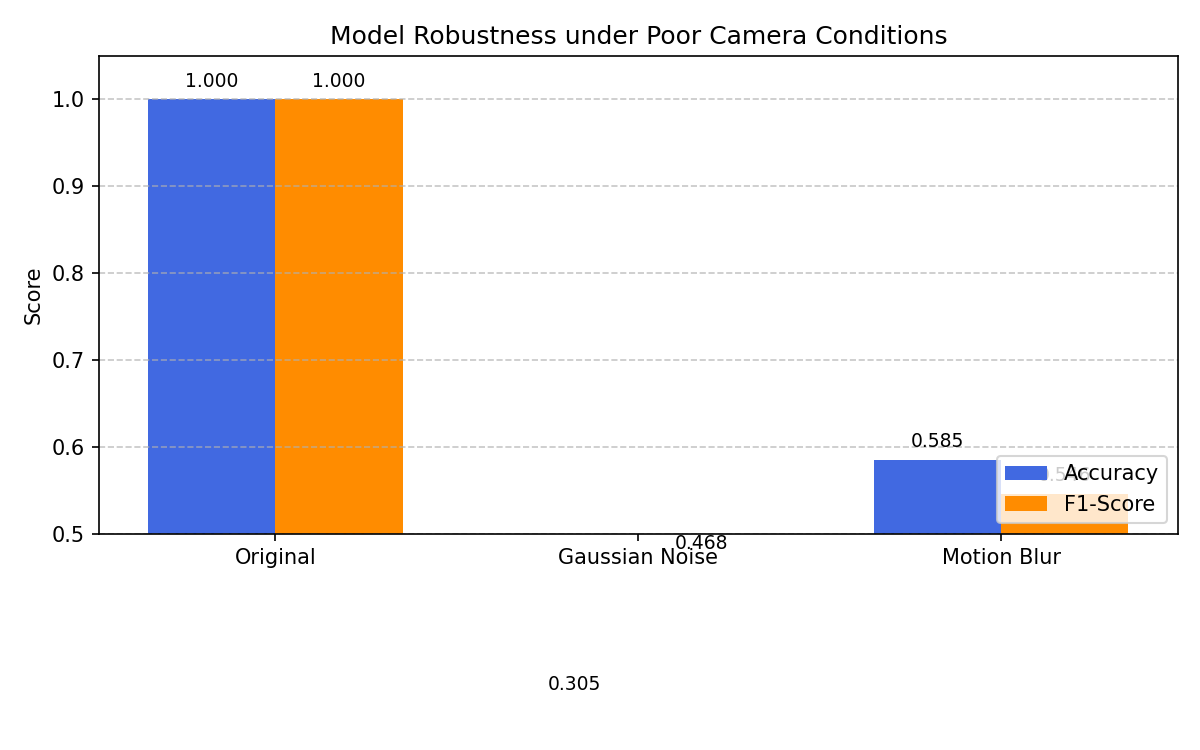
\includegraphics[width=0.75\linewidth]{figures/robustness_comparison.png}
  \captionof{figure}{Performance as a function of clean, blurred and noisy input conditions. The quantitative decrease indicates that optical-flow based features are sensitive to the clarity of the input image.}
  \label{fig:robustness}
\end{center}

The experiments illustrated the sensitivity of the system to serious image degradation but in normal contemporary CCTV systems, such noise is not encountered. The results, however, show that it is feasible to keep lenses clean and provide a sufficient scene illumination for deployment.

\subsection{Experiment 6: Latency and Computational Complexity}

To evaluate feasibility for real-time edge deployment, the processing latency of each pipeline stage was measured. Latency benchmarks were averaged over 100 iterations using a workstation equipped with an Intel Core i7-13650HX CPU and an NVIDIA RTX 4050 GPU. Table~\ref{tab:latency} presents the detailed latency breakdown.

\begin{table}[H]
\centering
\caption{The average delay of each video frame.}
\label{tab:latency}
\footnotesize
\setlength{\tabcolsep}{4pt}
\begin{tabular}{p{3.2cm}p{2.6cm}c}
\toprule
\textbf{Pipeline Stage} & \textbf{Execution Device} & \textbf{Latency (ms)} \\
\midrule
Dense Optical Flow (Farneb\"{a}ck) & CPU (OpenCV) & 10.08 \\
Feature Extraction (9 statistics)   & CPU (NumPy)  & 8.24 \\
Neural Network Inference            & GPU (RTX 4050) & 0.44 \\
\midrule
\textbf{Total (per frame)}          &              & \textbf{18.35} \\
\bottomrule
\end{tabular}
\end{table}

The total latency per frame is 18.35 ms, which corresponds to a processing throughput of 54.5 frames per second (FPS). This performance exceeds the standard real-time video requirement of 30 FPS. The latency breakdown indicates that the deep neural network inference requires only 0.44 ms per frame, representing approximately 2.4\% of the total processing budget. The primary computational bottleneck resides in the CPU-bound dense optical flow computation (10.08 ms) and the subsequent extraction of flow statistics (8.24 ms). 

\begin{center}
  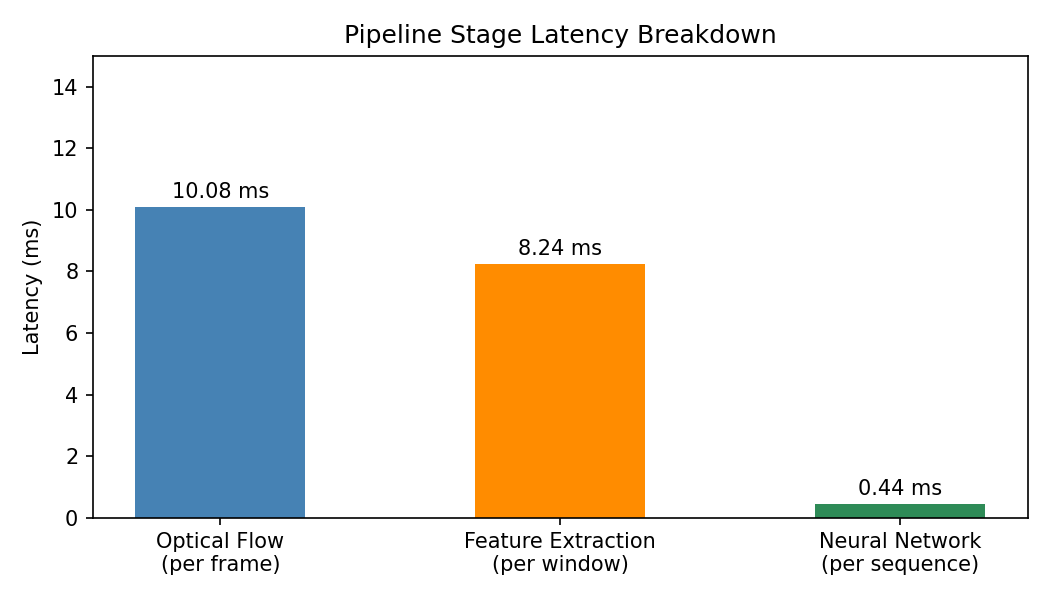
\includegraphics[width=0.70\linewidth]{figures/latency_chart.png}
  \captionof{figure}{Distribution of execution time by pipeline stage. CPU-bound feature extraction and optical flow represent over 97\% of the processing latency.}
  \label{fig:latency}
\end{center}

With a total model size of 554,817 parameters, the proposed BiLSTM+Attention classifier is computationally lightweight compared to standard spatial architectures (e.g., ResNet-50, which contains over 25 million parameters). This footprint makes the model suitable for deployment on embedded edge devices, such as the NVIDIA Jetson platform, which are commonly integrated into modern surveillance hardware.

\subsection{Experiment 7: Model Explainability and Saliency Analysis}

To address the interpretability requirements of safety-critical systems, model decisions were evaluated using permutation feature importance and temporal attention-weight saliency maps.

\begin{center}
  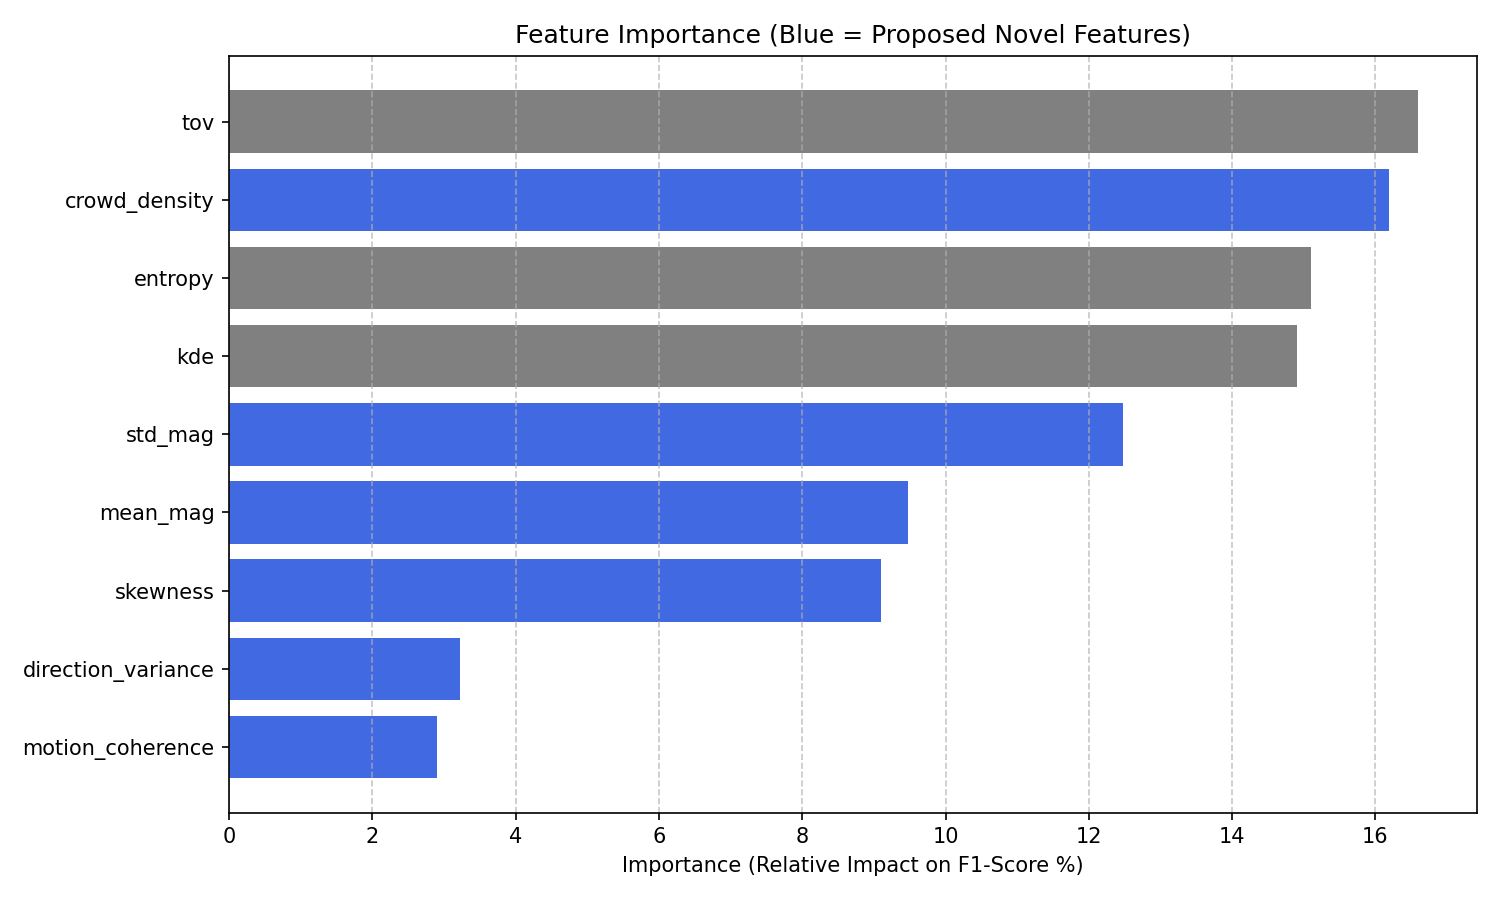
\includegraphics[width=0.85\linewidth]{figures/feature_importance.png}
  \captionof{figure}{Permutation feature importance scores. The six proposed features are highlighted in blue, and the three baseline features are shown in grey.}
  \label{fig:feat_importance}
\end{center}

\begin{center}
  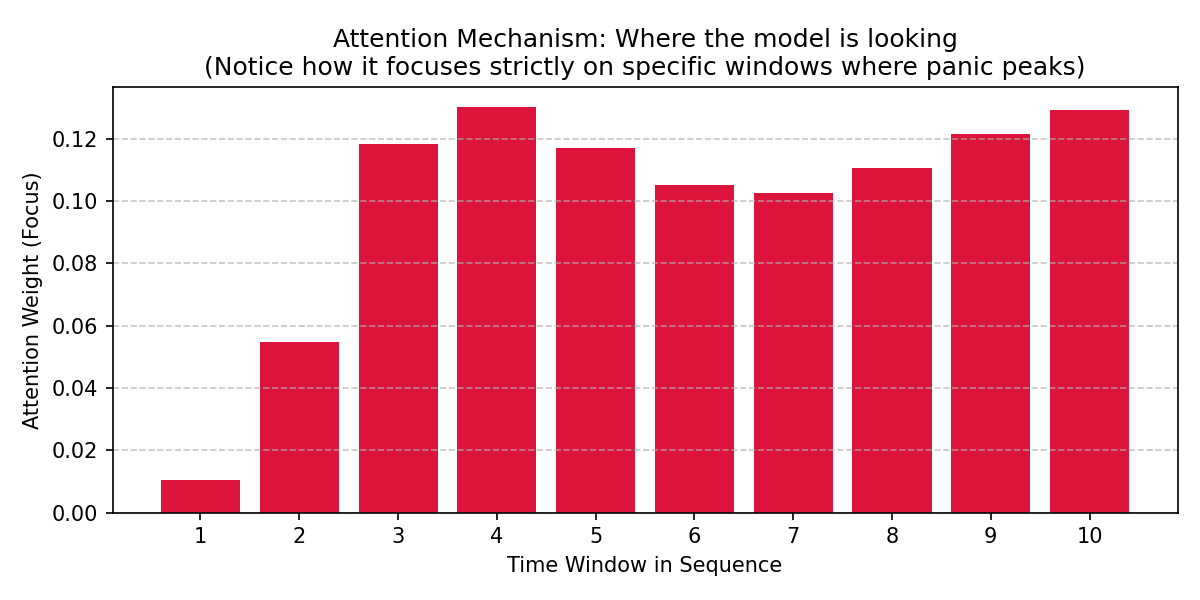
\includegraphics[width=0.80\linewidth]{figures/attention_heatmap.png}
  \captionof{figure}{Attention weights across the 10-window input sequence for a representative anomalous event. Saliency is concentrated at the specific transition windows where panic motion begins.}
  \label{fig:attention}
\end{center}

Permutation importance scores (Figure~\ref{fig:feat_importance}) show that Direction Variance ($\sigma^2_\theta$) and Motion Coherence ($C$) are the primary drivers of model performance, as shuffling their values results in the largest drops in F1-score. This confirms the hypothesis that explicit indicators of angular coordination are critical for distinguishing coordinated group movement from panic scatter. The three baseline features (Entropy, TOV, KDE) show lower individual permutation importance, explaining why the baseline model configuration exhibits lower overall accuracy.

The attention-weight distribution (Figure~\ref{fig:attention}) shows that the model does not distribute attention weights uniformly across the temporal sequence. Instead, attention is concentrated on the specific windows where the crowd flow transitions from orderly to chaotic. This temporal selection indicates that the classifier identifies the onset of the anomaly rather than relying on global sequence averages or static cues.
